\section{Results}

Implementation of the our approach is provided in the \texttt{R} package \href{https://dajmcdon.github.io/rtestim/}{\texttt{rtestim}}. 


\subsection{Experimental settings}

% problem settings
%% Rt
We consider four scenarios of the time-varying effective reproduction numbers. The first two scenarios are simple cases that are rapidly controlled by intervention, where the graphical curvatures consist of one knot and two segments, and the last two scenarios are more complicated, which involve more waves in the epidemics. Scenario 1 is instantaneous prior and post-intervention, and Scenario 2 is exponentially grow and decay. Scenario 3 has four constant segments with three knots, which reflect the effect of intervention, the resurge to large epidemic, and the suppression of pandemic respectively. Scenario 4 involves more complicated waves of the epidemic. 
%% other problem settings
We run experiments over 50 random samples for each setting. We consider all epidemics starting from 2 incidence cases and generating until timepoints 300. 
% 
To verify the performance of our model under the violation of distributional assumption of incidence, we generate incidence samples using negative Binomial distribution with dispersion size 5. The serial interval follows Gamma distribution with shapes and scales $(3,3)$, $(2.5,2.5)$, $(3.5,3.5)$ and $(3.5,3.5)$ for the four scenarios respectively. 
An example of each effective reproduction number scenario with corresponding Poisson and negative Binomial incidences are displayed in \autoref{fig:samples}. 

\begin{figure}[tb]
    \centering
    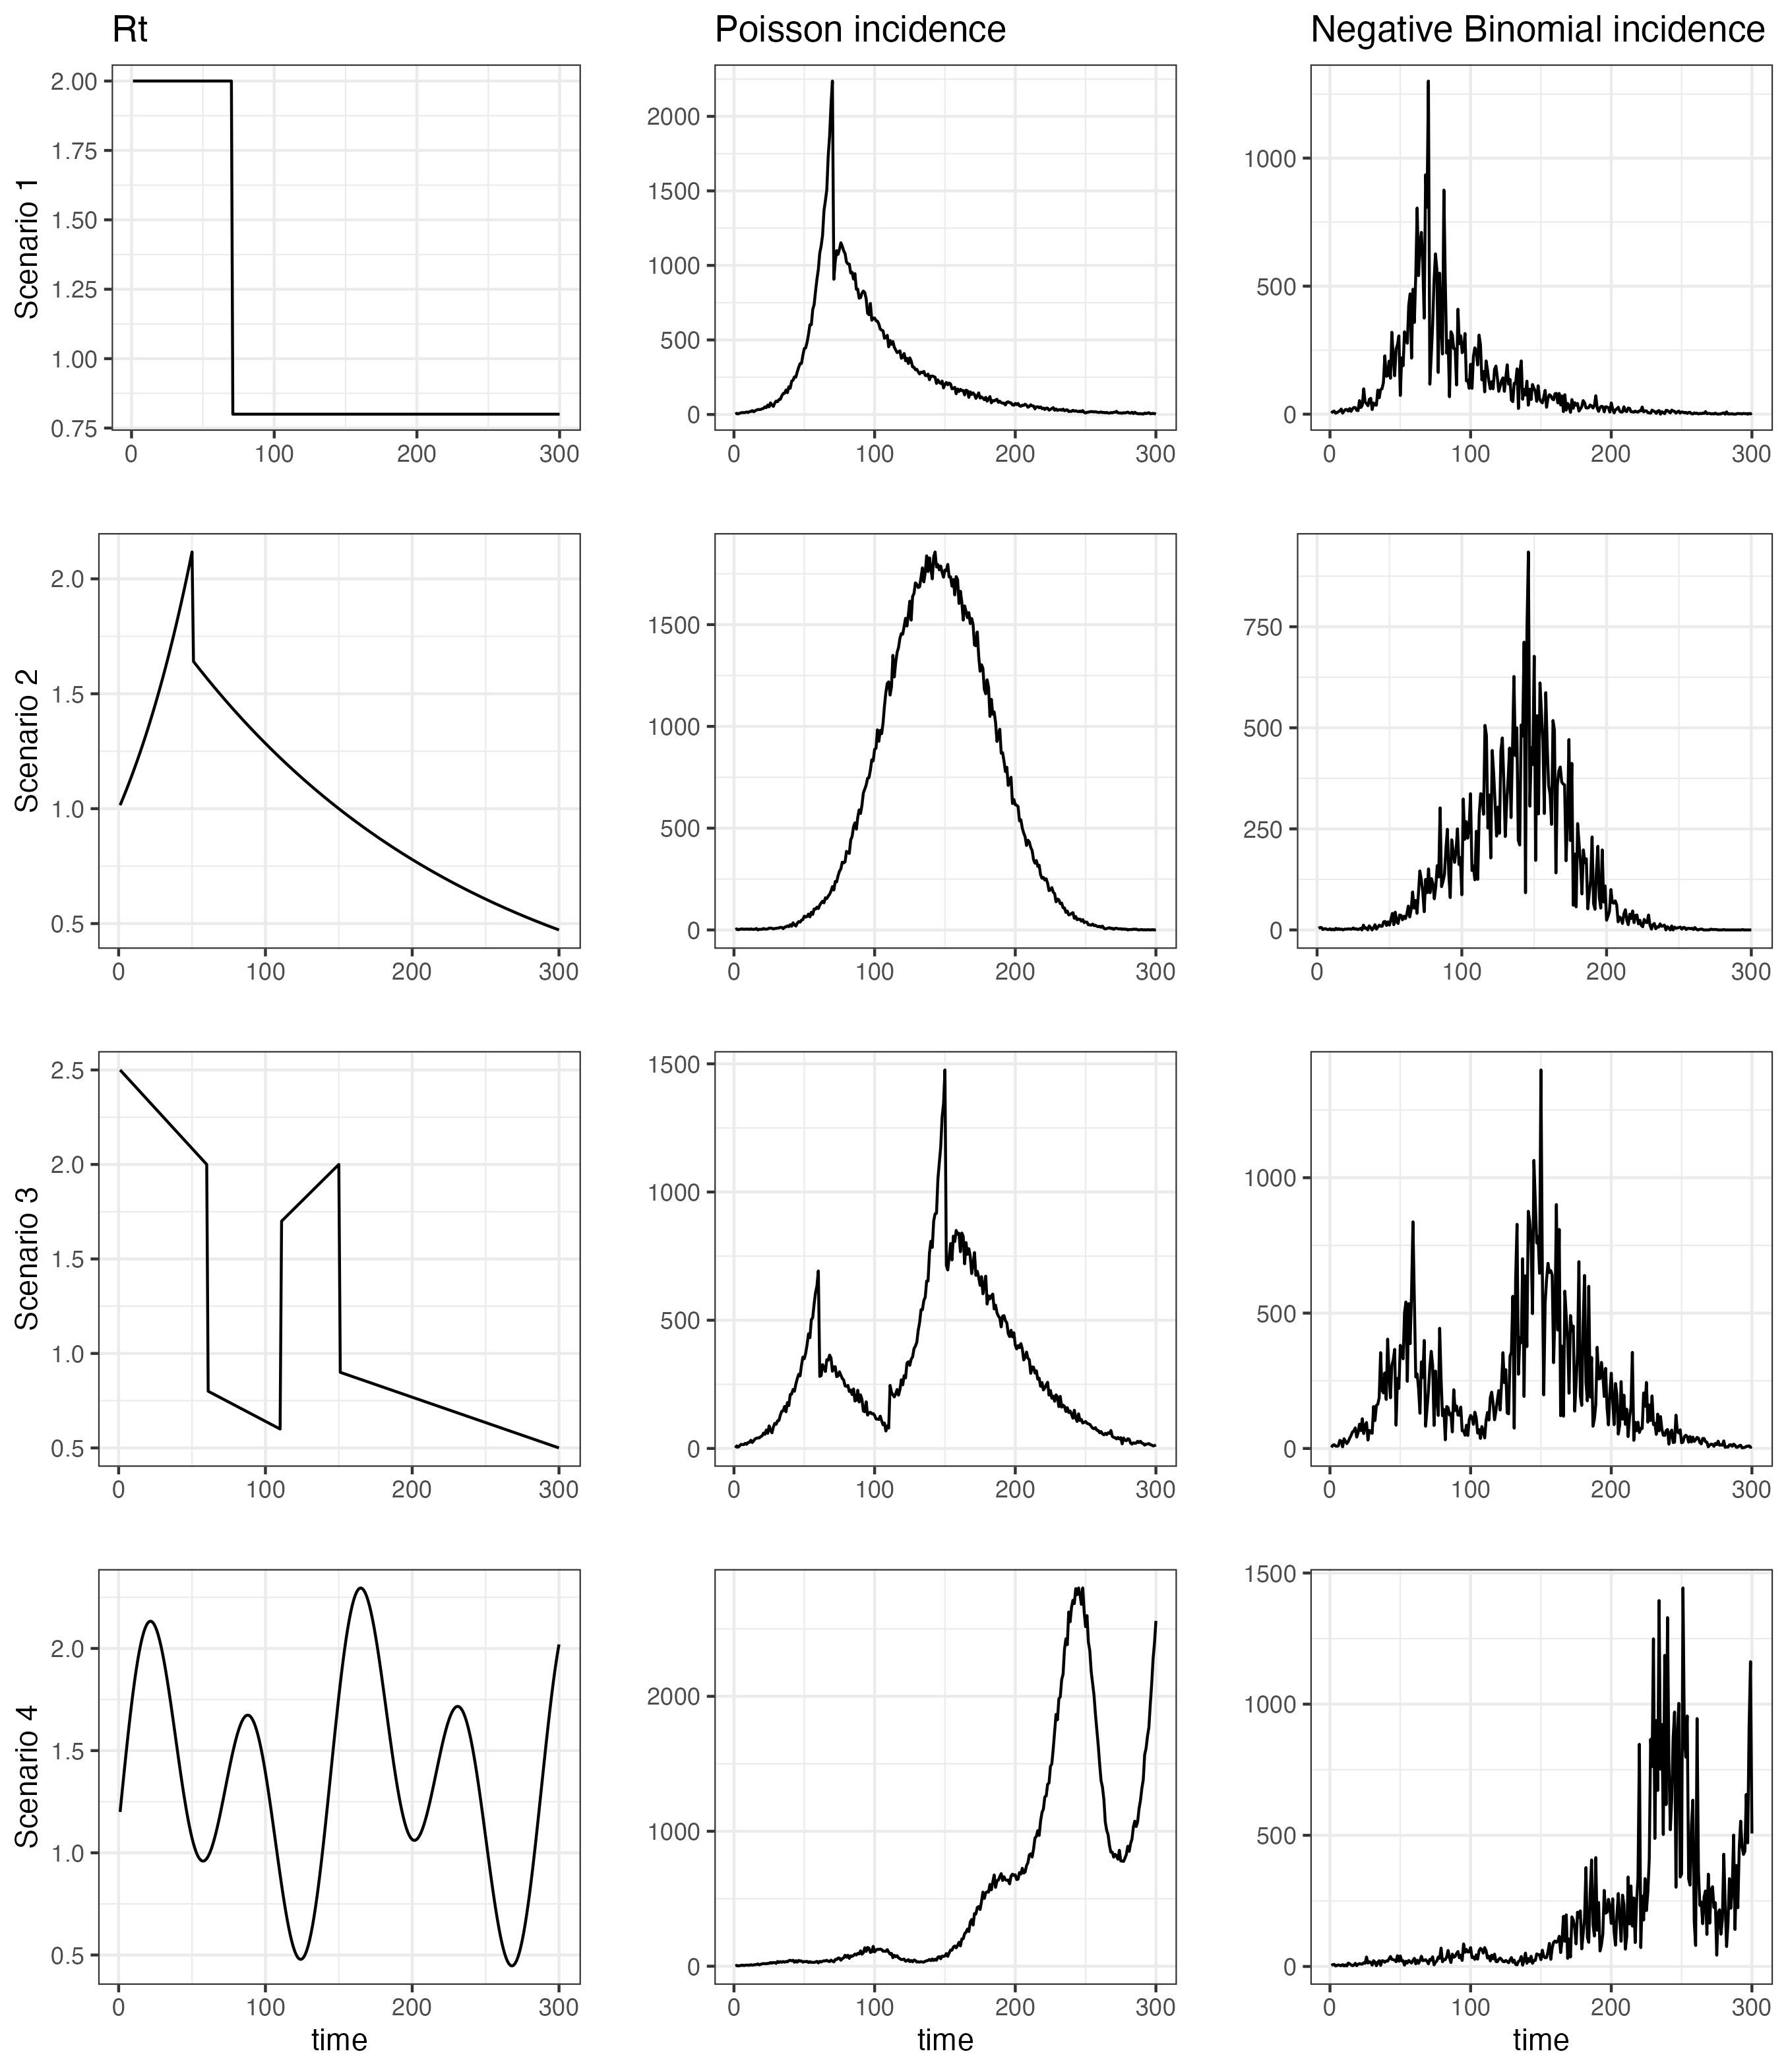
\includegraphics[width=140mm]{fig/plot_samples.png}
    \caption{An example of effective reproduction numbers and corresponding incidences following Poisson or negative Binomial distribution. The first column illustrates four $\calR_t$ cases. The second column is the Poisson incidences corresponding to the effective reproduction numbers. The third column is the negative Binomial distributed incidences for each $\calR_t$ case.}
    \label{fig:samples}
\end{figure}

% algorithm settings
%% our RtEstim
We tune the model over the candidate set of size 50 using cross validation. We use degrees $k=0,3,1,3$ for the four scenarios respectively. 
%% competitors and their settings
We compare our \RtEstim\ to \EpiEstim\ and \EpiLPS. \EpiEstim\ is a widely used Bayesian method that estimates the posterior distribution of effective reproduction numbers given the Gamma prior and Poisson distributed incidence. They estimate the reproduction number over a sliding window by assuming the reproduction number is constant during the specific time window. We use the default weekly sliding window. \EpiLPS\ is another Bayesian approach that estimates P-splines coupled with Laplace approximations of the conditional posterior of the spline vector based on negative Binomial distributed incidences. 
%
We assume the serial interval distributions are known for all models. 

The accuracy of $\calR_t$ estimates is measured by the mean Kullback-Leibler (KL) divergence for Poisson distributions, i.e., $$\frac{1}{n} D_{KL}(\hat{\calR}_{1:n}|| \calR_{1:n}) = \frac{1}{n}\sum_{t=1}^n \hat{\calR}_t \log\left(\frac{\hat{\calR}_t}{\calR_t}\right) + {\calR}_t - \hat{\calR}_t,$$ where $\calR_{1:n} := \left\{ \calR_t \right\}_{t=1}^n$. In comparison of the accuracy across methods, we drop the estimates during the first week as the $\calR_t$ estimates of \EpiEstim\ starts at $t=8$. 
Other details of the experiments are deferred to the supplementary document. 

\subsection{Experimental results}

% experiment results
\autoref{fig:pois-est} illustrates the estimated reproduction numbers by three models for the Poisson incidence cases. Compared to \EpiEstim\ and \EpiLPS, which have an edge problem at the beginning of the time series, our \RtEstim\ estimates are more accurate --- almost overlap with the true values --- and without suffering from the edge problem. Scenario 2 is a difficult problem for all methods; the immediate drop from an exponential growth to an exponential decay is hard to capture. Since we fit a cubic Poisson trend filtering problem for Scenario 2, our estimated $\hat{\calR}_t$ curve is continuous at the knot, which hinders the estimates from fitting the steep decline. 
Scenario 1 is the simplest case with only one knot and two constant segments. Besides the edge problem, \EpiEstim\ and \EpiLPS\ produce ``smooth'' estimated curves that are continuous at the knot, which results in divergence from the true values in the first segment in Scenario 1. Since the piecewise constant \RtEstim\ estimator is not continuous, it captures the sharp decrease in $\calR_t$ in Scenario 1. 
\begin{figure}[tb]
    \centering
    \includegraphics*[width=140mm]{fig/Pois-res-plot.png}
    \caption{Effective reproduction number estimation for Poisson incidences. Estimates of \EpiEstim\ during the first weeks are filled by the ``best'' cases, i.e., the first estimates at time $t=8$.}
    \label{fig:pois-est}
\end{figure}


% experiment results under the violation of assumptions
Under the violation of distributional assumption of incidences, we estimate $\calR_t$s using negative Binomial incidences. \autoref{fig:nb-est} displays the estimates over all methods. \RtEstim\ estimates overall do not perform as impressive as the Poisson incidence cases. Especially for Scenario 4, \RtEstim\ fails to recover the wiggly curvature during the first few waves. In Scenario 2, \RtEstim\ succeeds to capture the knot, but suffers from the same problem as in the Poisson cases. In Scenario 3, piecewise linear \RtEstim\ estimates fail to capture the knots and do not fit well during the first half of the time period. 
\begin{figure}[tb]
    \centering
    \includegraphics*[width=140mm]{fig/NB-res-plot.png}
    \caption{Effective reproduction number estimation for negative Binomial incidences. Estimates of \EpiEstim\ during the first weeks are filled by the ``best'' cases, i.e., the first estimates at time $t=8$.} 
    \label{fig:nb-est}
\end{figure}

The KL divergences are displayed in \autoref{fig:kl-res}. \RtEstim\ overall performs better than \EpiEstim\ and \EpiLPS. In Scenario 2, the KL divergence boxes of \EpiLPS\ is slightly lower than \RtEstim's boxes, but \EpiLPS\ has large outliers for both Poisson and negative Binomial incidences cases. In general, given the Poisson incidences, \RtEstim\ is more accurate than \EpiEstim\ and \EpiLPS\ across Scenarios 1, 3, 4, and slightly less accurate but more stable than \EpiLPS\ in Scenario 2. Given negative Binomial incidences, \RtEstim\ is still the most accurate in Scenarios 1 and 3, and achieves similar levels of accuracy as \EpiLPS\ in Scenarios 2 and 4. \RtEstim\ has larger outliers than \EpiLPS\ across all scenarios given negative Binomial incidences, but the difference is no more than $0.1$. 
\begin{figure}[htb]
    \centering
    \includegraphics*[width=160mm]{fig/kl.png}
    \caption{Boxplot of Kullback-Leibler divergence between the estimated effective reproduction numbers and the true ones across all methods given Poisson incidences and negative Binomial incidences across 50 samples. Left panel visualizes the KL divergences for the Poisson incidence cases. Right panel displays the KL divergences for the negative Binomial incidence cases.} 
    \label{fig:kl-res}
\end{figure}


\subsection{Covid-19 incidences in British Columbia}

% introduce data & hyperparameter setup
We implement the proposed model on the Covid-19 confirmed cases in British Columbia (B.C.) as of May 18, 2023 reported by B.C. Conservation Data Centre. We choose the gamma distribution with shape $2.5$ and scale $2.5$ to approximate the serial interval function. Covid-19 incidence cases are visualized in \autoref{fig:covid-data}.
\begin{figure}[tb]
    \centering
    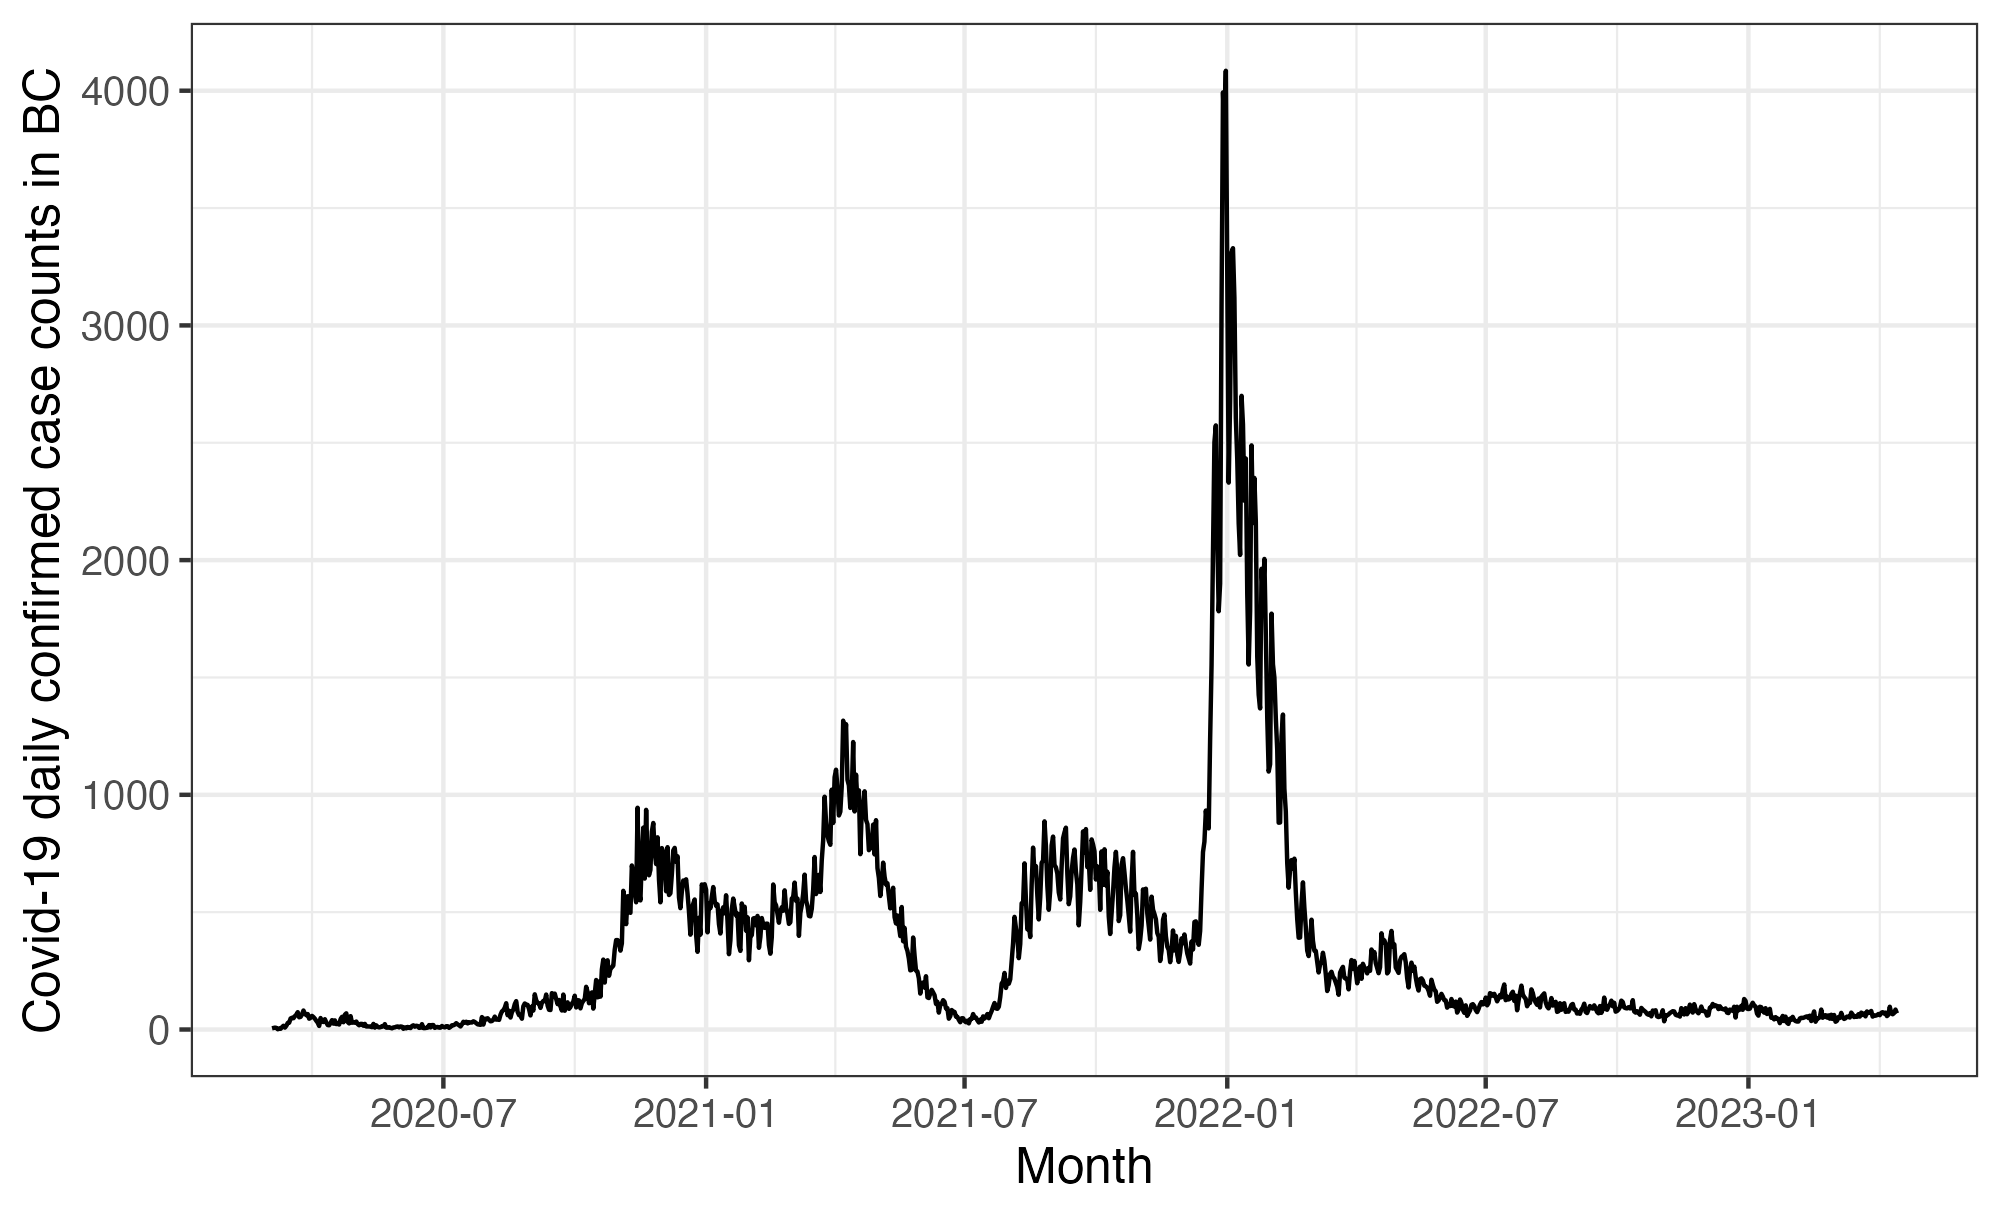
\includegraphics[width=0.99\linewidth]{fig/covid_dat.png}
    \caption{Covid19 daily confirmed incidence counts between March 1st, 2020 and April 15th, 2023 in British Columbia, Canada.} 
    \label{fig:covid-data}
\end{figure} 

% interpret figures -- across all lambdas
Considering the temporal evolutions of neighboring $3, 4, 5$ reproduction numbers, the estimated reproduction numbers of Covid-19 in British Columbia (illustrated in \autoref{fig:covid-res}) are less than $3$ during most of the time, which means that one distinct infected individuals can on average infect less than three other individuals in the population. The three degrees of the temporal evolution (across all regularization levels $\lambda$) all yield similar results that $\hat{\calR}_t$ achieves the highest peak around the end of 2021 and reaches the lowest trough shortly thereafter. Throughout the estimated curves, the peaks and troughs of the reproduction numbers roughly come prior to the following growths and decays of confirmed cases respectively.

The reproduction numbers are relatively unstable before April 1st, 2022. The highest peak coincides with the emergence and globally spread of the Omicron variant. The estimated reproduction numbers are apparently below the threshold $1$ during two time periods -- roughly from April 1st, 2021 to July 1st, 2021 and from January 1st, 2022 to April 1st, 2022. The first trough of $\hat{\calR}_t$ coincides with the first authorization for use of Covid-19 vaccines in British Columbia. The second trough shortly after the greatest peak may credit to many aspects, including self-isolation of the infected individuals and application of the second shot of Covid-19 vaccines. Since around April 1st, 2022, the reproduction numbers stay stable (fluctuating around $1$) and the infected cases stay low. 

% for different lambda
Greater regularization levels (i.e., larger $\lambda$s) result in smoother estimated curves. Smoother curves suggest that the estimated reproduction numbers are around $1$ during most time periods; however, they may not be appropriate to interpret the reality. More wiggly curves better reflect the fluctuation of $\calR_t$, but sometimes fail to highlight the significant peaks or troughs. The tuning parameter $\lambda$ needs to be chosen corresponding to the information in practice for a better interpretation. 
\begin{figure}[tb]
    \centering
    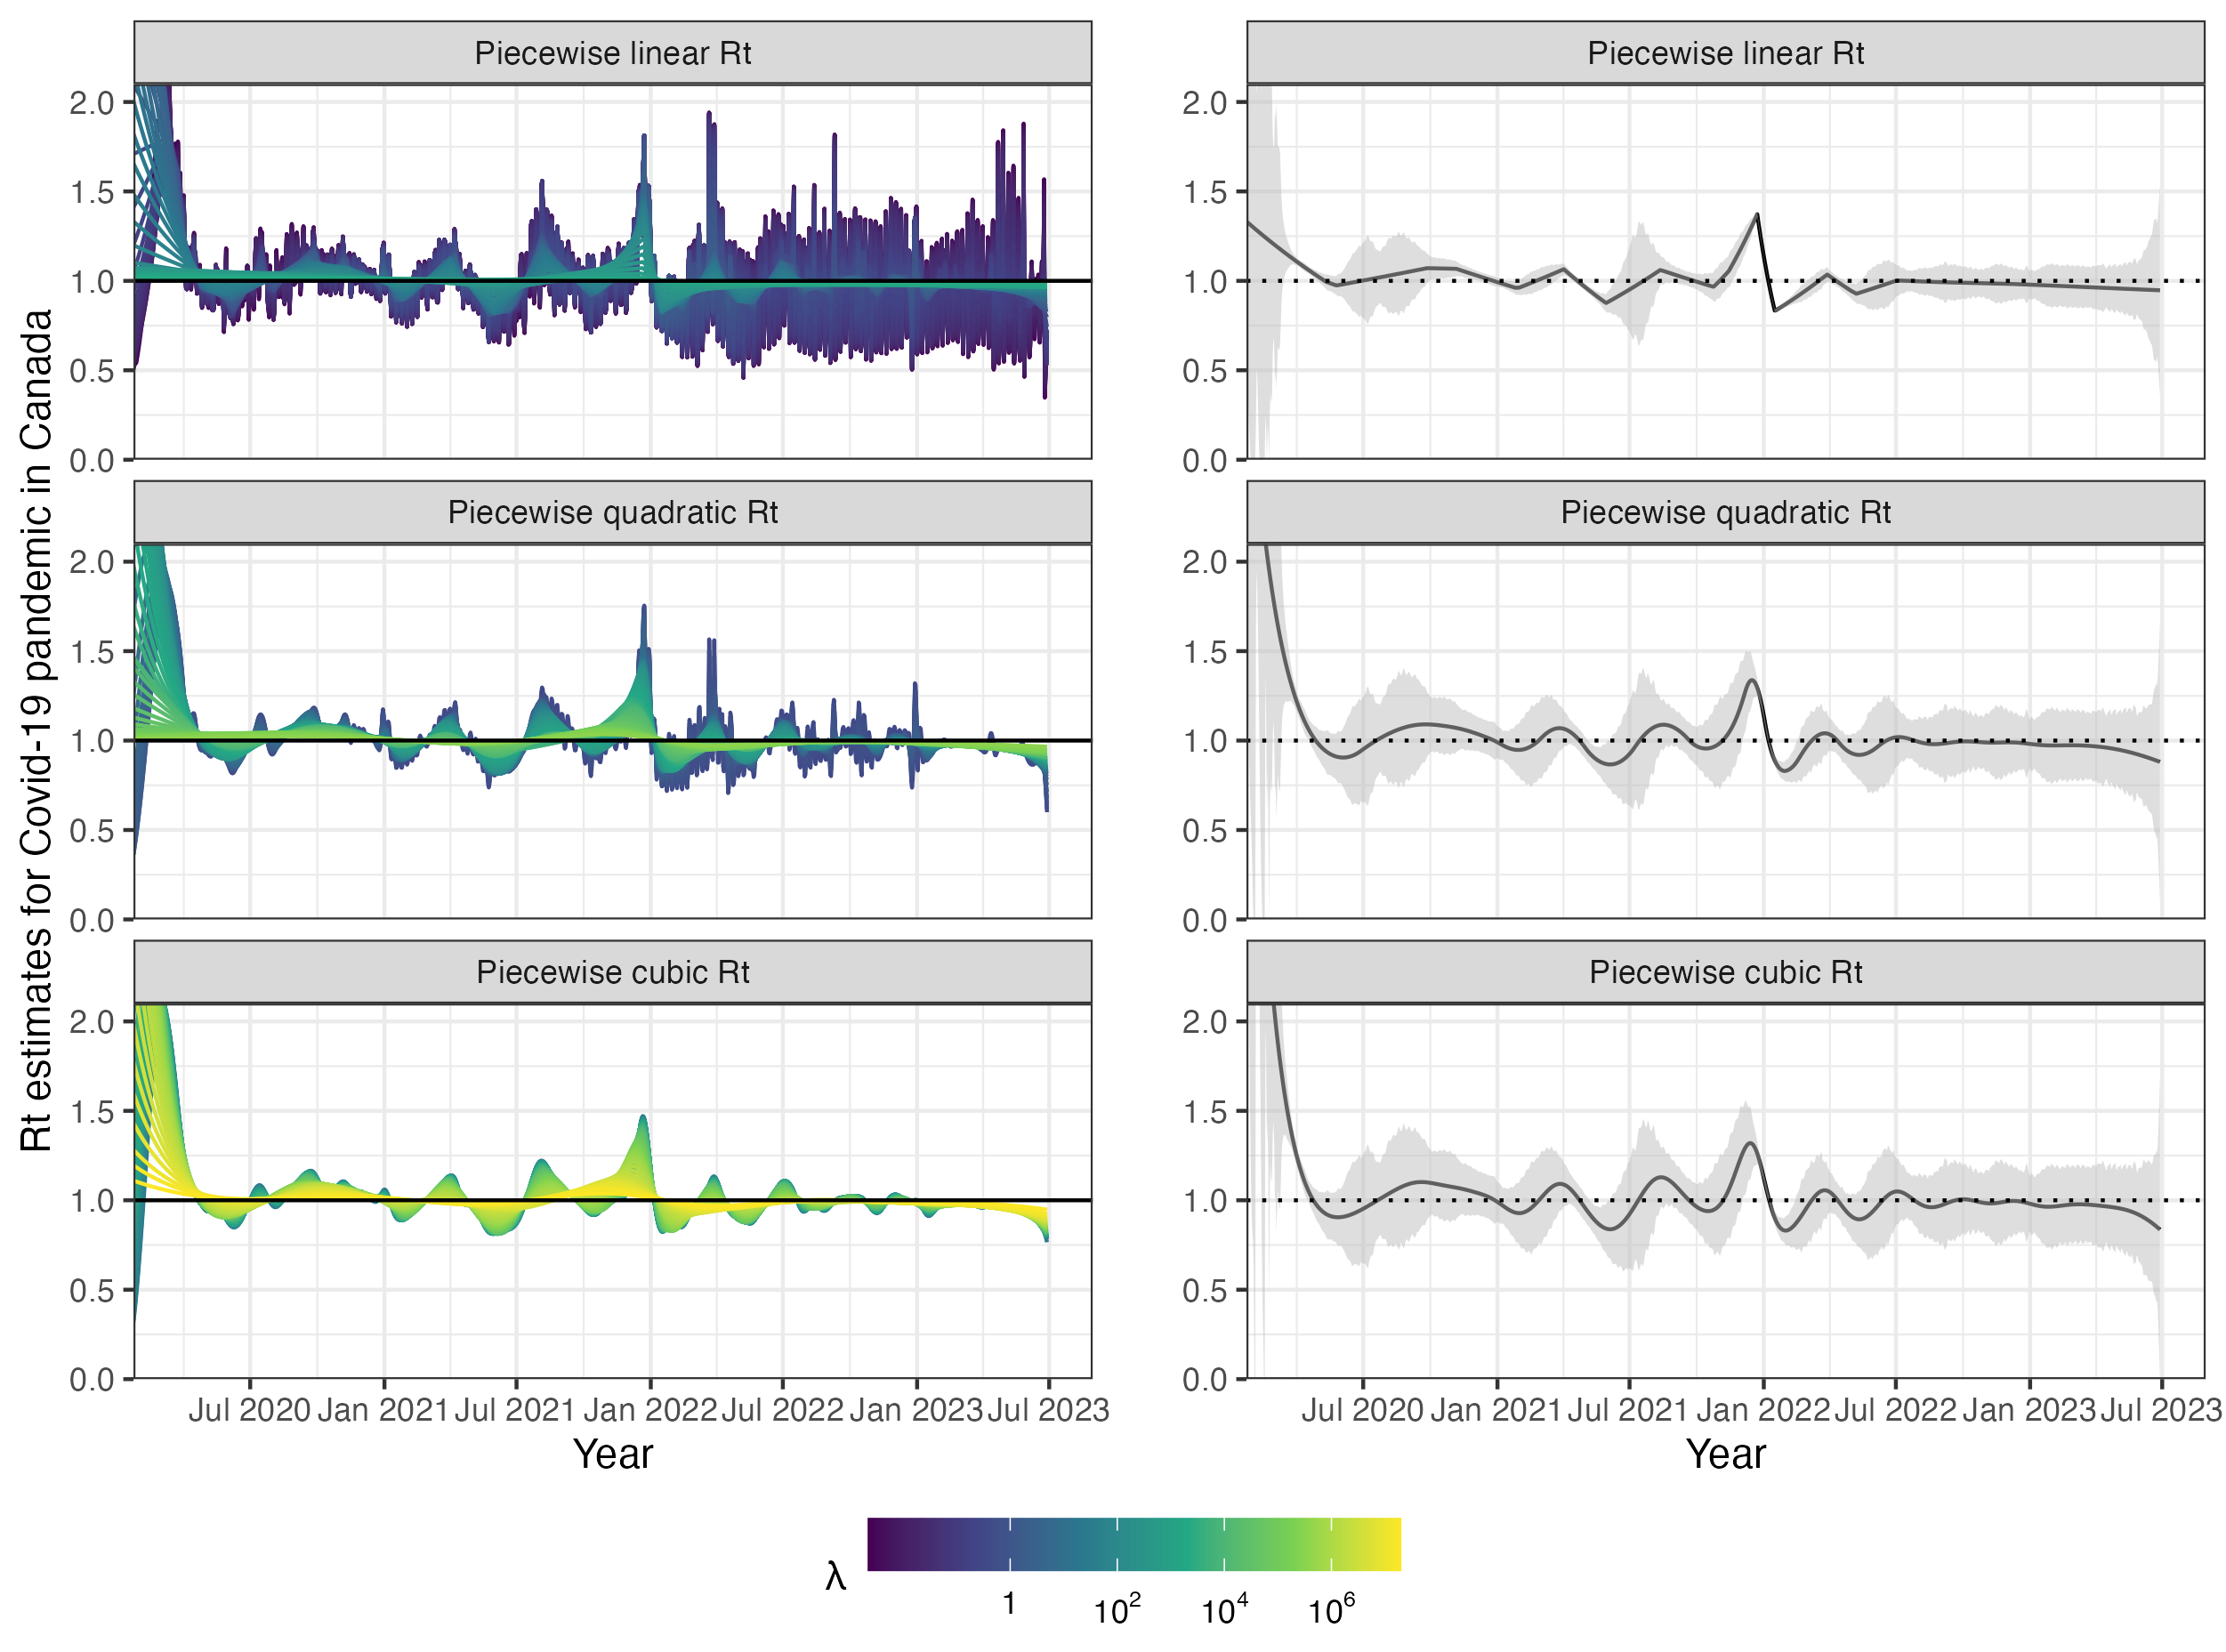
\includegraphics[width=0.99\linewidth]{fig/covid_full_res.png}
    \caption{Estimated effective reproduction numbers for Covid19 daily confirmed counts between March 1st, 2020 and April 15th, 2023 in British Columbia, Canada. The left panels display the CV-tuned estimates with 95\% confidence intervals. The right panels demonstrate estimates corresponding to 50 tuning parameters. The top, medium and bottom panels illustrate the estimated reproduction numbers ($\calR_t$) using the Poisson trend filtering (in \eqref{eq:rt-ptf}) with degrees $k=1,2,3$ respectively.} 
    \label{fig:covid-res}
\end{figure} 


\subsection{Pandemic influenza in Baltimore, Maryland, 1918}

We then apply \RtEstim\ on the pandemic influenza in Baltimore, Maryland, 1918. Dataset in \autoref{fig:flu-dat} is obtained from the \texttt{R} package \EpiEstim. In the estimation displayed in \autoref{fig:flu-res}, the CV-tuned piecewise cubic estimates better capture the growing tendency at the beginning of the pandemic. It suggests that the pandemic has yielded a decrease after around 20 days and reached $1$ when the pandemic has lasted for nearly 50 days. However, it also suggests an increase at the end of the period, while a steady decline (as in CV-tuned piecewise constant and linear estimates) is more reasonable. The smoothness of $\calR_t$ curves should be chosen based on the purpose of the study in practice, e.g., epidemic forecasting may require a more wiggly curve that contains more fluctuation information, while retrospective studies that solely target on understanding of the pandemic may prefer a smoother curve with less important information smoothed out. 
\begin{figure}[tb]
    \centering
    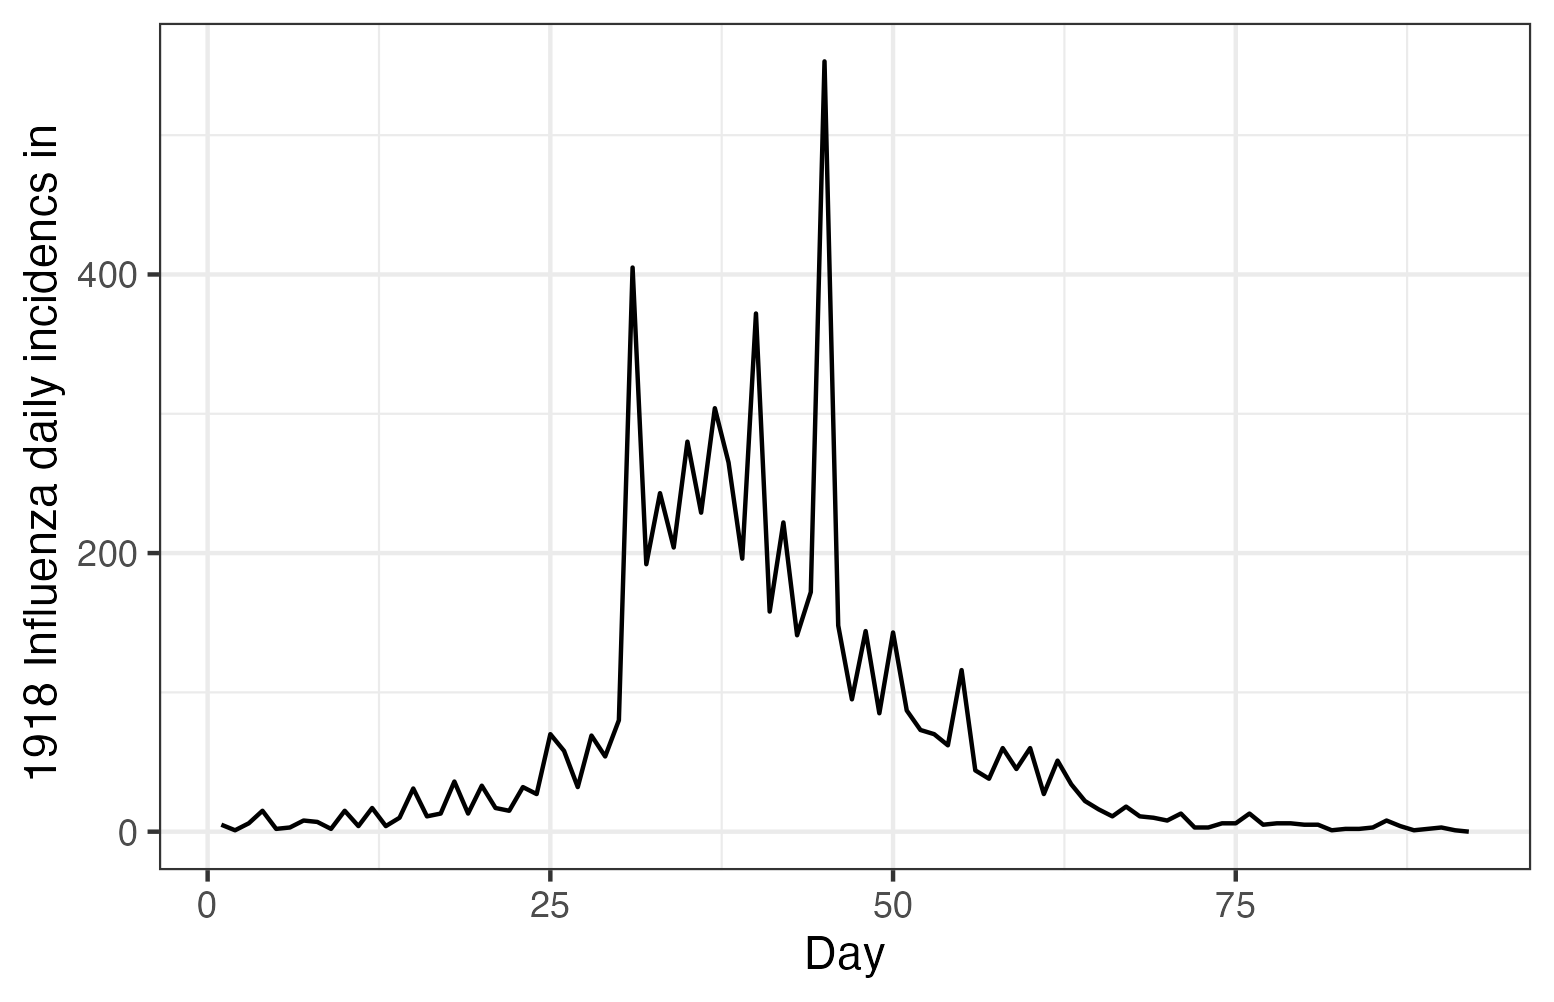
\includegraphics[width=0.9\linewidth]{fig/flu_dat.png}
    \caption{Pandemic influenza incidence counts in Baltimore, Maryland in 1918.} 
    \label{fig:flu-dat}
\end{figure} 

\begin{figure}[tb]
    \centering
    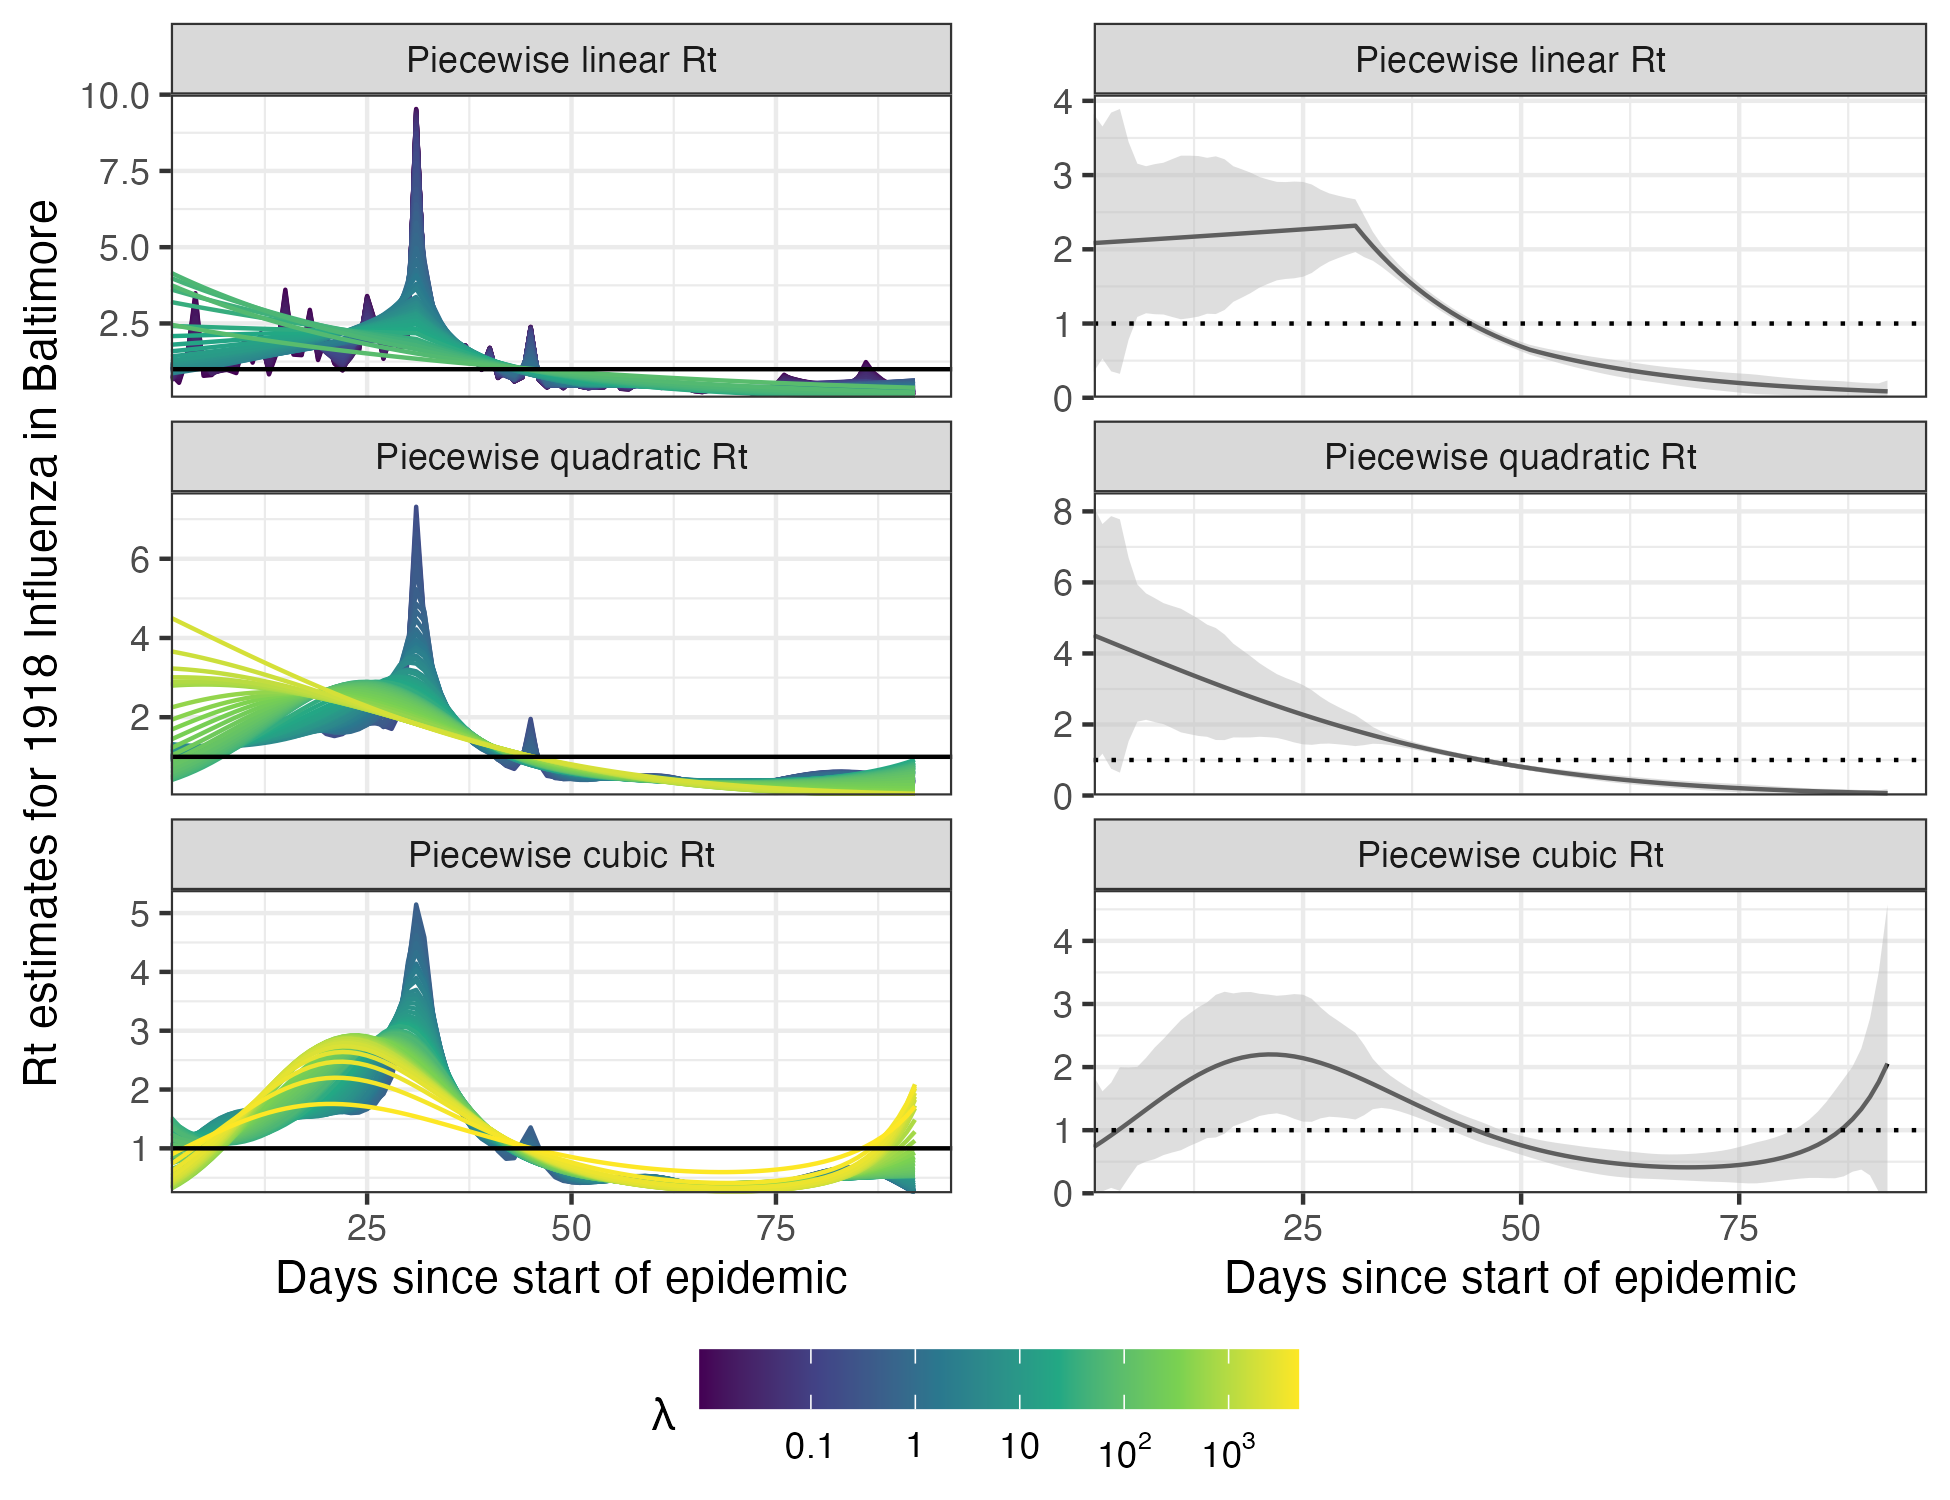
\includegraphics[width=0.9\linewidth]{fig/flu_full_res.png}
    \caption{Estimated effective reproduction numbers for pandemic influenza incidence counts in Baltimore, Maryland in 1918. The left panels display the CV-tuned estimates with 95\% confidence intervals. The right panels demonstrate estimates corresponding to 50 tuning parameters. The top, medium and bottom panels illustrate the estimated reproduction numbers ($\calR_t$) using the Poisson trend filtering (in \eqref{eq:rt-ptf}) with degrees $k=1,2,3$ respectively.} 
    \label{fig:flu-res}
\end{figure} 

